% Created 2023-10-20 Fri 09:07
% Intended LaTeX compiler: pdflatex
\documentclass[11pt,oneside]{memoir}
\makeatletter

\usepackage{answerkey-env}

\ifanswerkey
  \usepackage[forcolorpaper, answerkey]{eqexam}
  \usepackage{vinaya-class-questions}
\else
  \usepackage[forcolorpaper, nosolutions]{eqexam}
  \usepackage[nosolutions]{vinaya-class-questions}
\fi

\proofingsymbolColor{linkred}
\fillinColor{linkred}

\def\maketitle{}

\maxtocdepth{subsection}

\newenvironment{twocols}{%
  \raggedright%
  \setlength{\parindent}{0pt}%
  \setlength{\parskip}{8pt}%
  \fontsize{11}{17}\selectfont%
  \begin{multicols}{2}%
}{%
  \end{multicols}%
}

\newenvironment{widecols}{%
  \hspace*{-0.05\linewidth}\begin{minipage}{1.1\linewidth}%
  \raggedright%
  \setlength{\parindent}{0pt}%
  \setlength{\parskip}{8pt}%
  \fontsize{11}{17}\selectfont%
  \begin{multicols}{2}%
}{%
  \end{multicols}%
  \end{minipage}%
}

\newlength\@tmp@width
\newlength\@tmp@height

\renewcommand*{\printchaptertitleHook}{%
  \AddToShipoutPictureBG*{%
    \put(\LenToUnit{\paperwidth-25mm-\spinemargin},\LenToUnit{\paperheight-95mm}){%
      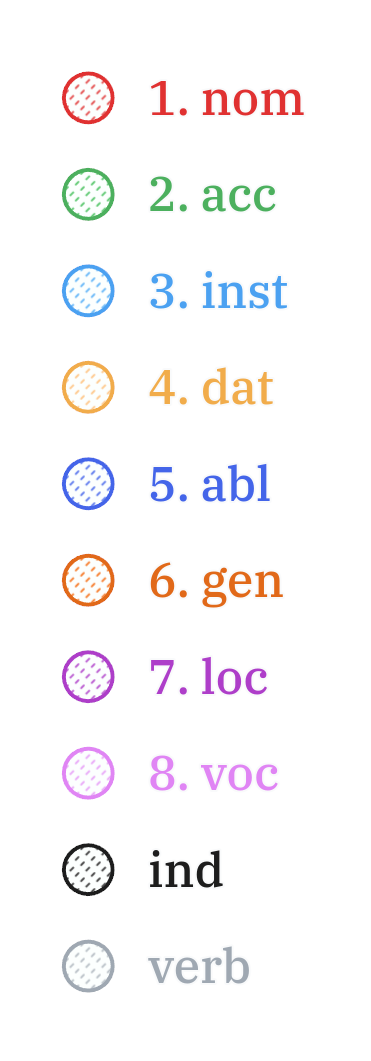
\includegraphics[width=25mm]{./images/cases-legend-white-large.png}%
    }%
  }%
}

\newcommand*\sentenceDiaMsg{\textbf{Exercise:} Draw a sentence analysis diagram below and indicate declensions.}

\newcommand*\sentenceDiaSolution[2][0.4]{%
  \ifanswerkey%
    \hspace*{-\spinemargin}%
    \begin{minipage}{\paperwidth}%
      \centering%
      \includegraphics[scale=#1]{#2}%
    \end{minipage}%
  \else%
    \settototalheight{\@tmp@height}{\includegraphics[scale=#1]{#2}}%
    \begin{minipage}[\@tmp@height]{\linewidth}%
      \sentenceDiaMsg%
    \end{minipage}%
  \fi%
}

\usepackage{cwpuzzle}

\renewcommand\PuzzleCluePre{%
  \begin{minipage}[t]{0.75\linewidth}%
}

\renewcommand\PuzzleClueFont{\fontsize{11}{17}\selectfont}

% \def\PuzzleThickline{\linethickness{2pt}}

\makeatother

\maxtocdepth{section}
\date{\today}
\title{Pali Readings}
\hypersetup{
 pdfauthor={The Bhikkhu Saṅgha},
 pdftitle={Pali Readings},
 pdfkeywords={},
 pdfsubject={},
 pdfcreator={Emacs 29.1 (Org mode 9.6.6)}, 
 pdflang={En_Gb}}
\begin{document}

\maketitle
\frontmatter

{\centering

{\Huge Pāḷi Readings}

\bigskip
\href{https://vinaya-class.github.io}{https://vinaya-class.github.io}

{\scshape\small last updated on}\\
\today

}

\bigskip
\tableofcontents*

\mainmatter

\yournamefalse

\newlength{\colOne}\setlength{\colOne}{0.35\linewidth}
\newlength{\colTwo}\setlength{\colTwo}{0.6\linewidth}

\renewenvironment{quote}%
{\list{}{%
    \doubleLineSize
    \listparindent 0pt
    \itemindent    0pt
    \leftmargin    3em
    \rightmargin   3em
    \parsep        0pt
    \topsep        8pt
    \partopsep     0pt}%
\item[] \raggedright}%
{\endlist}

\chapter{Ratana Sutta Paritta (Snp 2.1)}
\label{sec:org28388a5}

\begin{quote}
Yaṁ kiñci vittaṁ idha vā huraṁ vā, \\[0pt]
Saggesu vā yaṁ ratanaṁ paṇītaṁ; \\[0pt]
Na no samaṁ atthi tathāgatena, \\[0pt]
Idampi buddhe ratanaṁ paṇītaṁ; \\[0pt]
Etena saccena suvatthi hotu.
\end{quote}

\begin{longtable}{L{\colOne} L{\colTwo}}
yaṁ \ldots{} taṁ \ldots{} & what \ldots{} that \ldots{}\\[0pt]
yaṁ kiñci (ind.) [yaṁ + kiṁ + ci] & whatever; everything; all\\[0pt]
vitta (nt.) & (1) wealth; property (2) delight; pleasure; lit. got\\[0pt]
huraṁ (ind.) & there; in another world\\[0pt]
sagga (m.) & heaven; paradise\\[0pt]
ratana (nt.) & (1) jewel; gem (2) treasure (3) queen\\[0pt]
paṇīta (adj.) & fine; superior; sublime; lit. brought forward\\[0pt]
sama (adj.) & (1) level; even; balanced (2) like; equal (to); same (as)\\[0pt]
sacca (nt.) & truth\\[0pt]
suvatthi (f.) [su + √as + ti] & well being; prosperity\\[0pt]
\end{longtable}

\begin{quote}
Khayaṁ virāgaṁ amataṁ paṇītaṁ, \\[0pt]
Yadajjhagā sakyamunī samāhito; \\[0pt]
Na tena dhammena samatthi kiñci, \\[0pt]
Idampi dhamme ratanaṁ paṇītaṁ; \\[0pt]
Etena saccena suvatthi hotu.
\end{quote}

\enlargethispage{\baselineskip}

\begin{longtable}{L{\colOne} L{\colTwo}}
khīyati & is destroyed; is exhausted\\[0pt]
khīṇa (pp. of khīyati) & consumed; destroyed\\[0pt]
khaya (m. from khīyati) & wearing away; destruction\\[0pt]
virāga (m.) & fading of desire (for); dispassion (towards)\\[0pt]
amata (nt.) & (1) deathless state; immortality (2) deathless; immortal; undying\\[0pt]
adhigacchati & gets to; attains; obtains; lit. arrives at\\[0pt]
ajjhagā (imperf. of adhigacchati) & got; obtained; achieved; lit. arrived at\\[0pt]
samādahati & (1) (of the mind) composes; stabilizes; collects (2) (of fire) kindles; lights; lit. puts together\\[0pt]
samāhita (pp. of samādahati) & composed; centred; settled\\[0pt]
\end{longtable}

\clearpage

\begin{quote}
Yaṁ buddhaseṭṭho parivaṇṇayī suciṁ, \\[0pt]
Samādhimānantarikaññamāhu; \\[0pt]
[samādhiṁ + ānantarikaṁ + yaṁ + āhu] \\[0pt]
Samādhinā tena samo na vijjati, \\[0pt]
Idampi dhamme ratanaṁ paṇītaṁ; \\[0pt]
Etena saccena suvatthi hotu.
\end{quote}

\begin{longtable}{L{\colOne} L{\colTwo}}
seṭṭha (adj.) & (1) foremost; supreme; (2) chief; leader\\[0pt]
vaṇṇayati & (1) praises; extols (2) comments on; interprets; explains\\[0pt]
parivaṇṇayati & describes; recommends; extolls; lit. praises all around\\[0pt]
suci (adj.) & (1) clean; pure (2) (of tastes and smells) good; fine\\[0pt]
antara (nt.) & space between; interval; distance\\[0pt]
ānantarika (adj.) & immediate; without delay; with immediate results\\[0pt]
√ah & (√) speak\\[0pt]
āhu (perf.3rd.pl. of āha) & they say; lit. they said\\[0pt]
vijjati [√vid + ya + ti] & (1) exists; is found; is present (2) is possible\\[0pt]
\end{longtable}

\begin{quote}
Ye puggalā aṭṭha sataṁ pasatthā, \\[0pt]
Cattāri etāni yugāni honti; \\[0pt]
Te dakkhiṇeyyā sugatassa sāvakā, \\[0pt]
Etesu dinnāni mahapphalāni; \\[0pt]
Idampi saṅghe ratanaṁ paṇītaṁ, \\[0pt]
Etena saccena suvatthi hotu.
\end{quote}

\begin{longtable}{L{\colOne} L{\colTwo}}
ye \ldots{} te \ldots{} & who \ldots{} they \ldots{}\\[0pt]
puggala (m.) & person; individual\\[0pt]
santa (m. irreg, from atthi) & virtuous man; good person (from √as)\\[0pt]
sataṁ (m.dat.pl. of santa, irreg) & for virtuous people; for good people\\[0pt]
pasaṁsati & praises; approves (of); commends\\[0pt]
pasattha (pp. of pasaṁsati) & praised; commended; exalted\\[0pt]
yuga (nt.) & (1) yoke (2) pair; set of two\\[0pt]
dadāti & gives (to); offers (to)\\[0pt]
dinna (pp. of dadāti) & given (to); offered (to)\\[0pt]
phala (nt.) & (1) fruit; berry (2) consequence; result\\[0pt]
\end{longtable}

\clearpage

\begin{quote}
Ye suppayuttā manasā daḷhena, \\[0pt]
Nikkāmino gotamasāsanamhi; \\[0pt]
Te pattipattā amataṁ vigayha, \\[0pt]
Laddhā mudhā nibbutiṁ bhuñjamānā; \\[0pt]
Idampi saṅghe ratanaṁ paṇītaṁ, \\[0pt]
Etena saccena suvatthi hotu.
\end{quote}

\begin{longtable}{L{\colOne} L{\colTwo}}
payuñjati & harnesses; employs; applies\\[0pt]
payutta (pp. of payuñjati) & intent; engaged\\[0pt]
suppayutta (adj.) [su + payutta] & fully engaged; diligently practising\\[0pt]
manasa (adj.) & focused on; lit. with such a mind\\[0pt]
daḷha (adj.) & strong; firm; steady\\[0pt]
nikkāmī (adj.) [nī + √kam + *ī] & striving (in); active (in); lit. going out\\[0pt]
pāpuṇāti & reaches; attains; arrives (at)\\[0pt]
patti (f. abstr. from pāpuṇāti) & (1) reaching; getting (2) profit; share; lit. what is obtained\\[0pt]
patta (pp. of pāpuṇāti) & reached; attained; have arrived (at)\\[0pt]
vigāhati & enters, plunges into\\[0pt]
vigayha (ger. of vigāhati) & plunging into; diving into\\[0pt]
labhati & gets; receives; obtains\\[0pt]
laddhā (abs. of labhati) & having got; having obtained\\[0pt]
mudhā (ind.) & for free; freely; gratis; for nothing\\[0pt]
nibbuti (f.) [nī + √vā + ti] & quenching; cooling; lit. blown away state\\[0pt]
bhuñjamāna (prp. of bhuñjati) & eating; consuming; enjoying\\[0pt]
\end{longtable}

\clearpage

\begin{quote}
Khīṇaṁ purāṇaṁ navaṁ natthi sambhavaṁ, \\[0pt]
Virattacittāyatike bhavasmiṁ; \\[0pt]
Te khīṇabījā avirūḷhichandā, \\[0pt]
Nibbanti dhīrā yathāyaṁ padīpo; \\[0pt]
Idampi saṅghe ratanaṁ paṇītaṁ, \\[0pt]
Etena saccena suvatthi hotu.
\end{quote}

\begin{longtable}{L{\colOne} L{\colTwo}}
khīyati & is destroyed; is exhausted\\[0pt]
khīṇa (pp. of khīyati) & consumed; destroyed\\[0pt]
khaya (m. from khīyati) & wearing away; destruction\\[0pt]
purāṇa (adj.) & previous; old; ancient\\[0pt]
nava (adj.) & new; fresh\\[0pt]
sambhavati & comes to be; happens; occurs\\[0pt]
sambhava (m. from sambhavati) & birth; origin; source (of)\\[0pt]
rajjati & finds pleasure (in); is enamoured (with)\\[0pt]
virajjati & becomes detached (from); loses interest (in)\\[0pt]
viratta (pp. of virajjati) & detached (from); without desire (for); lost interest (in)\\[0pt]
āyati (f.) & future; upcoming\\[0pt]
āyatika (adj. from āyati) & upcoming; future\\[0pt]
bīja (nt.) & seed; germ\\[0pt]
virūḷhi (f.) & growth; increase\\[0pt]
chanda (m.) & (1) interest; desire; wish (2) consent; agreement\\[0pt]
nibbāti & is extinguished; goes out; lit. blows away\\[0pt]
dhīra (adj.) & (1) stable; constant; reliable; firm (2) wise; intelligent\\[0pt]
padīpa (m.) & lamp; light; lighting\\[0pt]
\end{longtable}

\chapter{Paṭhamabhavasutta (AN 3.76)}
\label{sec:org9141169}

(\href{https://suttacentral.net/an3.76/pli/ms}{AN 3.76})

\begin{quote}
Atha kho āyasmā ānando yena bhagavā tenupasaṅkami; upasaṅkamitvā bhagavantaṁ
abhivādetvā ekamantaṁ nisīdi. Ekamantaṁ nisinno kho āyasmā ānando bhagavantaṁ
etadavoca:
\end{quote}

\begin{longtable}{L{\colOne} L{\colTwo}}
yena \ldots{} ten'upasaṅkamati (idiom) & wherever \ldots{} he approaches (him/it)\\[0pt]
abhivādeti & bows down (to); pays high respect (to)\\[0pt]
anta (m.) & end; side; extreme\\[0pt]
ekamantaṁ (ind.) [ekaṁ + anta + aṁ] & to one side; aside\\[0pt]
vacati & speaks\\[0pt]
avoca (aor. of vacati) & said (to)\\[0pt]
\end{longtable}

\begin{quote}
“bhavo, bhavo'ti, bhante, vuccati. Kittāvatā nu kho, bhante, bhavo hotī”ti?

“Kāmadhātuvepakkañca, ānanda, kammaṁ nābhavissa, api nu kho kāmabhavo paññāyethā”ti?

“No hetaṁ, bhante”.
\end{quote}

\begin{longtable}{L{\colOne} L{\colTwo}}
bhava (m.) & being; becoming; existence\\[0pt]
vuccati (pass. of vacati) & is said to be; is called\\[0pt]
tāva (ind.) & that much; that far; still; at least\\[0pt]
kittāvatā (ind.) [ka + tāva + tā] & in what way?; to what extent?\\[0pt]
dhātu (f.) & (1) state; property; condition (2) state of being; realm of existence\\[0pt]
kāmadhātu (f.) & realm of desire; world of sense pleasure\\[0pt]
√pac & (√) cook; mature; ripen\\[0pt]
vipaccati [vi + √pac + ya + ti] & bears fruit; gives results\\[0pt]
vipakka (pp. of vipaccati) & ripened; matured; given fruit\\[0pt]
vepakka (nt. from vipakka) & ripening; maturing; bearing fruit\\[0pt]
nābhavissa [na + abhavissa] & would not exist\\[0pt]
pajānāti & knows clearly; understands; distinguishes\\[0pt]
paññāyati (pass. of pajānāti) & is clearly known; is evident\\[0pt]
paññāyetha (opt.reflx.3rd.sg. of paññāyeyya) & it itself would be evident; it could be discerned\\[0pt]
\end{longtable}

\clearpage

\begin{quote}
“Iti kho, ānanda, kammaṁ khettaṁ, viññāṇaṁ bījaṁ, taṇhā sneho. Avijjānīvaraṇānaṁ
sattānaṁ taṇhāsaṁyojanānaṁ hīnāya dhātuyā viññāṇaṁ
patiṭṭhitaṁ\footnote{: \href{https://suttacentral.net/an3.77/en/sujato}{AN 3.77}: cetanā patiṭṭhitā patthanā patiṭṭhitā} evaṁ āyatiṁ punabbhavābhinibbatti hoti. (…)
\end{quote}

\begin{longtable}{L{\colOne} L{\colTwo}}
khetta (nt.) & field; plot of land\\[0pt]
sneha (m.) & moisture\\[0pt]
nīvaraṇa (m.) & obstacle; obstruction; hindrance; lit. blocking\\[0pt]
satta (m.) [√as + a + tta] & being; living being; creature\\[0pt]
saṁyojana (nt.) & fetter; chain; bond; lit. yoking together\\[0pt]
hīna (adj.) & low; inferior; deficient\\[0pt]
cetanā (f.) [√cit + *anā] & intending; willing\\[0pt]
patthanā (f.) & intending; wishing; aspiring; praying; longing\\[0pt]
patiṭṭhahati [pati + √ṭhā + a + ti] & establishes; sets up; lit. stands before\\[0pt]
patiṭṭhita (pp. of patiṭṭhahati) & firmly grounded (in); well established (in)\\[0pt]
āyati (f.) & future; what's coming\\[0pt]
punabbhava (m.) & appearing again; renewed existence; rebirth; future life\\[0pt]
abhinibbatti (f.) & birth; becoming; production\\[0pt]
\end{longtable}

\begin{quote}
Rūpadhātuvepakkañca, ānanda, kammaṁ nābhavissa, api nu kho rūpabhavo
paññāyethā”ti?

“No hetaṁ, bhante”.

“Iti kho, ānanda, kammaṁ khettaṁ, viññāṇaṁ bījaṁ, taṇhā sneho. Avijjānīvaraṇānaṁ
sattānaṁ taṇhāsaṁyojanānaṁ majjhimāya dhātuyā viññāṇaṁ patiṭṭhitaṁ evaṁ āyatiṁ
punabbhavābhinibbatti hoti. (…)

Arūpadhātuvepakkañca, ānanda, kammaṁ nābhavissa, api nu kho arūpabhavo
paññāyethā”ti?

“No hetaṁ, bhante”.

“Iti kho, ānanda, kammaṁ khettaṁ, viññāṇaṁ bījaṁ, taṇhā sneho. Avijjānīvaraṇānaṁ
sattānaṁ taṇhāsaṁyojanānaṁ paṇītāya dhātuyā viññāṇaṁ patiṭṭhitaṁ evaṁ āyatiṁ
punabbhavābhinibbatti hoti. Evaṁ kho, ānanda, bhavo hotī”ti.
\end{quote}

\chapter{Cundīsutta (AN 5.32)}
\label{sec:orge07c57f}

(\href{https://suttacentral.net/an5.32/en/sujato}{AN 5.32}, also in \href{https://suttacentral.net/iti90/en/thanissaro}{Iti 90}, \href{https://suttacentral.net/an4.34/en/sujato}{AN 4.34})

\begin{quote}
Ekaṁ samayaṁ bhagavā rājagahe viharati veḷuvane kalandakanivāpe. Atha kho cundī
rājakumārī pañcahi rathasatehi pañcahi ca kumārisatehi parivutā yena bhagavā
tenupasaṅkami; upasaṅkamitvā bhagavantaṁ abhivādetvā ekamantaṁ nisīdi. Ekamantaṁ
nisinnā kho cundī rājakumārī bhagavantaṁ etadavoca:
\end{quote}

\begin{longtable}{L{\colOne} L{\colTwo}}
veḷuvana (nt.) [veḷu + vana] & Bamboo Grove, a park outside Rājagaha; lit. bamboo forest\\[0pt]
kalandaka (m.) & squirrel\\[0pt]
nivāpa (m.) & bait; fodder; feeding\\[0pt]
kumāra (m.) & young boy; prince\\[0pt]
kumārī (f.) & young girl; princess\\[0pt]
ratha (m.) & chariot; coach; carriage\\[0pt]
kumārisata (nt.) & one hundred maidens\\[0pt]
parivāreti & surrounds, follows\\[0pt]
\end{longtable}


\vspace*{-2\baselineskip}
\enlargethispage{2\baselineskip}

\begin{quote}
“Amhākaṁ, bhante, bhātā cundo nāma rājakumāro, so evamāha:

‘yadeva so hoti itthī vā puriso vā
buddhaṁ saraṇaṁ gato, dhammaṁ saraṇaṁ gato, saṅghaṁ saraṇaṁ gato,
pāṇātipātā paṭivirato, adinnādānā paṭivirato, kāmesumicchācārā paṭivirato,
musāvādā paṭivirato, surāmerayamajjapamādaṭṭhānā paṭivirato,
so kāyassa bhedā paraṁ maraṇā sugatiṁyeva upapajjati, no duggatin’ti.
\end{quote}

\begin{longtable}{L{\colOne} L{\colTwo}}
bhātar (m.) & brother\\[0pt]
yadeva [yaṁ + eva] & any; whichever\\[0pt]
itthī (f.) & woman; female\\[0pt]
saraṇa (nt.) & shelter; refuge; help; lit. going to\\[0pt]
ramati & enjoys; finds pleasure (in)\\[0pt]
paṭiviramati [pati + vi + √ram + a + ti] & abstains (from); refrains (from); shuns; avoids\\[0pt]
paṭivirata (pp. of paṭiviramati) & abstained (from); desisted (from)\\[0pt]
bheda (m.) & (1) death (2) schism; split; lit. breakup\\[0pt]
maraṇa (nt.) & death; dying\\[0pt]
sugati (f.) & good destination; happy fate; heaven; lit. going well\\[0pt]
upapajjati & is reborn (in); re-arises (in); lit. goes towards\\[0pt]
duggati (f.) & state of misery; bad destination; hell; lit. going badly\\[0pt]
\end{longtable}

\clearpage

\begin{quote}
Sāhaṁ, bhante, bhagavantaṁ pucchāmi:

‘kathaṁrūpe kho, bhante, satthari pasanno
kāyassa bhedā paraṁ maraṇā sugatiṁyeva upapajjati, no duggatiṁ?
Kathaṁrūpe dhamme pasanno \ldots{}
Kathaṁrūpe saṅghe pasanno \ldots{}
Kathaṁrūpesu sīlesu paripūrakārī \ldots{} no duggatin’”ti?
\end{quote}

\begin{longtable}{L{\colOne} L{\colTwo}}
sāhaṁ [sā + ahaṁ] & then I; and I\\[0pt]
pucchati & asks; enquires; questions\\[0pt]
kathaṁrūpa & what kind?\\[0pt]
satthari (m.) [√sās + tar + i] & in the teacher; in the master\\[0pt]
sīla (nt.) & (1) ethical/moral conduct; virtue (2) behaviour; habit\\[0pt]
paripūra (adj.) & full; filled up; complete\\[0pt]
paripūrakārī (adj.) [paripūra + kārī] & who completely fulfils\\[0pt]
\end{longtable}

\begin{quote}
“Yāvatā, cundi, sattā apadā vā dvipadā vā catuppadā vā bahuppadā vā rūpino vā
arūpino vā saññino vā asaññino vā nevasaññināsaññino vā,
tathāgato tesaṁ aggamakkhāyati arahaṁ sammāsambuddho.
Ye kho, cundi, buddhe pasannā, agge te pasannā.
Agge kho pana pasannānaṁ aggo vipāko hoti.
\end{quote}

\begin{longtable}{L{\colOne} L{\colTwo}}
yāvatā (ind.) [yāva + tā] & as long as; as far as; of all; to the extent that\\[0pt]
pada (nt.) & (1) foot (2) path; track; way\\[0pt]
sañjānāti & knows; perceives; conceives\\[0pt]
saññī (adj. from sañjānāti) & percipient (of); conscious (of)\\[0pt]
tesaṁ (pron.) [ta + esānaṁ] & for them; to them; to those; among them\\[0pt]
agga (adj.) & highest; supreme\\[0pt]
akkhāti & says (to); tells (to); explains (to)\\[0pt]
akkhāyati (pass. of akkhāti) & is considered; is said to be\\[0pt]
vipāka (m.) [vi + √pac + *a] & result; outcome; consequence; fruit; lit. ripening\\[0pt]
\end{longtable}

\clearpage

\begin{quote}
Yāvatā, cundi, dhammā saṅkhatā, ariyo aṭṭhaṅgiko maggo tesaṁ aggamakkhāyati.
Ye, cundi, ariye aṭṭhaṅgike magge pasannā, agge te pasannā.
Agge kho pana pasannānaṁ aggo vipāko hoti.

Yāvatā, cundi, dhammā saṅkhatā vā asaṅkhatā vā, virāgo tesaṁ aggamakkhāyati,
yadidaṁ -- madanimmadano pipāsavinayo ālayasamugghāto vaṭṭupacchedo taṇhākkhayo
virāgo nirodho nibbānaṁ.
Ye kho, cundi, virāge dhamme pasannā, agge te pasannā.
Agge kho pana pasannānaṁ aggo vipāko hoti.

Yāvatā, cundi, saṅghā vā gaṇā vā, tathāgatasāvakasaṅgho tesaṁ aggamakkhāyati,
yadidaṁ -- cattāri purisayugāni aṭṭha purisapuggalā, esa bhagavato sāvakasaṅgho
āhuneyyo pāhuneyyo dakkhiṇeyyo añjalikaraṇīyo anuttaraṁ puññakkhettaṁ lokassa.
Ye kho, cundi, saṅghe pasannā, agge te pasannā.
Agge kho pana pasannānaṁ aggo vipāko hoti.
\end{quote}

\begin{longtable}{L{\colOne} L{\colTwo}}
saṅkhata (pp. of saṅkharoti) & created; constructed; conditioned; fabricated; lit. put together\\[0pt]
mada (m.) [√mad + a] & (1) excess; pleasure; indulgence (2) vanity; pride; conceit\\[0pt]
nimmadana (nt.) [nir + √mad + ana] & removing pride; crushing conceit; lit. de-intoxicating\\[0pt]
pipāsa (adj.) & thirsty; lit. wishing to drink\\[0pt]
pipāsavinaya (m.) & removal of thirst\\[0pt]
ālaya (m.) & (1) roost; perch; nest; home (2) attachment (to); clinging (to)\\[0pt]
samugghāteti & abolishes, uproots, removes\\[0pt]
samugghāta (m. from samugghāteti) & eradication; extermination; destruction\\[0pt]
vaṭṭa (nt.) & (1) circle (2) cycle of existence; lit. round\\[0pt]
vaṭṭupaccheda (m.) & breaking off cycle of existence\\[0pt]
gaṇa (m.) & group; crowd\\[0pt]
sāvaka (m.) & disciple; pupil; follower\\[0pt]
\end{longtable}

\clearpage

\begin{quote}
Yāvatā, cundi, sīlāni, ariyakantāni sīlāni tesaṁ aggamakkhāyati, yadidaṁ --
akhaṇḍāni acchiddāni asabalāni akammāsāni bhujissāni viññuppasatthāni
aparāmaṭṭhāni samādhisaṁvattanikāni.
Ye kho, cundi, ariyakantesu sīlesu paripūrakārino, agge te paripūrakārino.
Agge kho pana paripūrakārīnaṁ aggo vipāko hotī'ti.
\end{quote}

\begin{longtable}{L{\colOne} L{\colTwo}}
kanta (adj.) & charming; pleasant; desirable; agreeable\\[0pt]
khaṇḍeti & breaks into pieces, transgresses\\[0pt]
akhaṇḍa (adj. from na khaṇḍeti) & unbroken; unfragmented; whole\\[0pt]
chindati & cuts off; severs\\[0pt]
acchidda (adj. from na chindati) & unbroken; flawless; without cracks\\[0pt]
sabala (adj.) & spotted; blotchy; mottled; patchy\\[0pt]
kammāsa (adj.) & spotted; speckled; blemished\\[0pt]
bhujissa (adj.) & cleansing; freeing; liberating\\[0pt]
pasaṁsati & praises; approves (of); commends\\[0pt]
pasattha (pp. of pasaṁsati) & praised; commended; exalted\\[0pt]
parāmasati & touches; strokes; rubs\\[0pt]
aparāmaṭṭha (pp. of na parāmasati) & irreproachable; untouchable; untarnished; lit. not touched\\[0pt]
saṁvattanika (adj.) & leading (to); headed (to); conducive (to)\\[0pt]
\end{longtable}

\begin{quote}
Aggato ve pasannānaṁ, \\[0pt]
aggaṁ dhammaṁ vijānataṁ; \\[0pt]
Agge buddhe pasannānaṁ, \\[0pt]
dakkhiṇeyye anuttare.
\end{quote}

\begin{longtable}{L{\colOne} L{\colTwo}}
agga (adj.) & highest; supreme\\[0pt]
pasāda (m.) & inspiration; faith; trust; confidence; lit. settling\\[0pt]
pasanna (adj.) & who has faith (in); who has confidence (in); lit. settled\\[0pt]
vijānāti & comprehends; understands\\[0pt]
vijānataṁ (prp. of vijānāti) & for those knowing; for those who understand\\[0pt]
dakkhiṇā (f.) & gift; donation\\[0pt]
dakkhiṇeyya (adj.) & worthy of offerings\\[0pt]
anuttara (adj.) & highest; unsurpassed; incomparable; lit. nothing higher\\[0pt]
\end{longtable}

\clearpage

\begin{quote}
Agge dhamme pasannānaṁ, \\[0pt]
virāgūpasame sukhe; \\[0pt]
Agge saṅghe pasannānaṁ, \\[0pt]
puññakkhette anuttare.
\end{quote}

\begin{longtable}{L{\colOne} L{\colTwo}}
virāga (m.) & fading of desire (for); dispassion (towards)\\[0pt]
upasamati & becomes calm; ceases; is allayed\\[0pt]
puñña (nt.) & merit; good deed; spiritual wealth\\[0pt]
khetta (nt.) & field; plot of land\\[0pt]
puññakkhetta (nt.) & field of merit\\[0pt]
\end{longtable}

\begin{quote}
Aggasmiṁ dānaṁ dadataṁ, \\[0pt]
aggaṁ puññaṁ pavaḍḍhati; \\[0pt]
Aggaṁ āyu ca vaṇṇo ca, \\[0pt]
yaso kitti sukhaṁ balaṁ.
\end{quote}

\begin{longtable}{L{\colOne} L{\colTwo}}
dadāti & gives; offers; donates\\[0pt]
dadanta (prp. of dadāti) & giving; offering; bestowing\\[0pt]
pavaḍḍhati & increases; develops; grows\\[0pt]
āyu (nt.) & life; longevity; age\\[0pt]
vaṇṇa (m.) & beauty; good looks; colour; appearance; lit. cover\\[0pt]
yasas (m.) & fame; reputation; renown\\[0pt]
kitti (f.) & fame; renown; celebrity\\[0pt]
\end{longtable}

\clearpage

\begin{quote}
Aggassa dātā medhāvī, \\[0pt]
aggadhammasamāhito; \\[0pt]
Devabhūto manusso vā, \\[0pt]
aggappatto pamodatī”ti.
\end{quote}

\begin{longtable}{L{\colOne} L{\colTwo}}
dātar (m.) & giver; donor; who gives\\[0pt]
medhā (f.) & wisdom; intelligence\\[0pt]
medhāvī (m.) & intelligent man; wise man; lit. who has wisdom\\[0pt]
samāhita (pp. of samādahati) & composed; centred; settled\\[0pt]
samāhita (adj. in comps.) & having; who has; endowed (with)\\[0pt]
patta (pp. of pāpuṇāti) & reached; attained; have arrived (at)\\[0pt]
pamodati & is delighted (with); is very happy (with)\\[0pt]
modati [√mud + *a + ti] & is happy; enjoys himself; rejoices\\[0pt]
muditā (f.) [√mud + ita + ā] & happiness (for); appreciation\\[0pt]
\end{longtable}

\clearpage

\section{Exercises}
\label{sec:org4657b44}

\renewcommand{\arraystretch}{1.6}

\begin{longtable}{l}
The Blessed One is staying in Rājagaha.\\[0pt]
\fillin{12cm}{bhagavā rājagahe viharati}\\[0pt]
Cundī princess (\emph{rājakumārī}) to the Blessed One said this \ldots{}\\[0pt]
\fillin{12cm}{cundī rājakumārī bhagavantaṁ etadavoca ...}\\[0pt]
My (\emph{amhākaṁ}) brother, called Cunda, the prince, he said this \ldots{}\\[0pt]
\fillin{12cm}{Amhākaṁ bhātā cundo nāma rājakumāro, so etadavoca / evamāha ...}\\[0pt]
A woman (\emph{itthī}) or man (who) has gone (\emph{gato}) to refuge to the Buddha.\\[0pt]
\fillin{12cm}{itthī vā puriso vā buddhaṁ saraṇaṁ gato}\\[0pt]
the break-up of the body, after death\\[0pt]
\fillin{12cm}{kāyassa bhedā paraṁ maraṇā}\\[0pt]
at heaven (\emph{sugati}) he appears / arises\\[0pt]
\fillin{12cm}{sugatiṁ upapajjati}\\[0pt]
I ask / enquire to the Blessed One \ldots{}\\[0pt]
\fillin{12cm}{Ahaṁ bhagavantaṁ pucchāmi ...}\\[0pt]
the best (\emph{agga}) result / outcome\\[0pt]
\fillin{12cm}{aggo vipāko}\\[0pt]
the things (which are) created / conditioned or uncreated / unconditioned\\[0pt]
\fillin{12cm}{dhammā saṅkhatā vā asaṅkhatā vā}\\[0pt]
dispassion is considered (\emph{akkhāyati}) the best\\[0pt]
\fillin{12cm}{virāgo aggamakkhāyati}\\[0pt]
the craving-destruction\\[0pt]
\fillin{12cm}{taṇhākkhayo}\\[0pt]
the incomparable merit-field of the world\\[0pt]
\fillin{12cm}{anuttaraṁ puññakkhettaṁ lokassa}\\[0pt]
they fulfil (into, \emph{loc.}) the moral precepts\\[0pt]
\fillin{12cm}{te sīlesu paripūrenti}\\[0pt]
confident / faithful in the best teaching\\[0pt]
\fillin{12cm}{agge dhamme pasannānaṁ}\\[0pt]
\end{longtable}

\normalArrayStrech

\chapter{Indulgence in Pleasure (1)}
\label{sec:org3741a86}
\section{Two Kinds of Pleasant Feeling}
\label{sec:orgd375f96}

\begin{quote}
Sāmisaṁ vā sukhaṁ vedanaṁ vedayamāno ‘sāmisaṁ sukhaṁ vedanaṁ vedayāmī’ti pajānāti.

Nirāmisaṁ vā sukhaṁ vedanaṁ vedayamāno ‘nirāmisaṁ sukhaṁ vedanaṁ vedayāmī’ti pajānāti. (\href{https://suttacentral.net/dn22/pli/ms}{DN 22})
\end{quote}

\begin{longtable}{L{\colOne} L{\colTwo}}
sāmisa (adj.) [sa + āma + isa] & carnal; material; worldly; lit. with raw meat\\[0pt]
nirāmisa (adj.) [nir + āma + isa] & not wordly; non-physical; spiritual\\[0pt]
\end{longtable}

\section{Pāsādikasutta (DN 29)}
\label{sec:org8d28d5b}

After the leader of the Jain sect, Nigaṇṭha Nāṭaputta died, his disciples are
arguing and quarreling. Their lay supporters are disappointed in them and with a
teaching poorly explained.

Ven. Ānanda and the novice Cunda goes to tell the Buddha about it.

He explains the various shortcomings of an incomplete spiritual path. One is fortunate
(\emph{lābhā}) if one turns away from it. He explains the advantages of a complete
teaching. One is fortunate if one practises following that system of training.

Spiritual companions (\emph{sabrahmacārī}) should recite the teachings together
(\emph{saṅgāyitabbadhamma}). They should reach agreement on correct understanding
through discussion (\emph{saññāpetabbavidhi}).

The Buddha gave teachings and made certain requisites allowable for the purpose of
restrining defilements in the present and future.

\begin{quote}
Diṭṭhadhammikānaṁ cevāhaṁ, cunda, āsavānaṁ saṁvarāya dhammaṁ desemi;
samparāyikānañca āsavānaṁ paṭighātāya.
\end{quote}

The Jain practice is characterized by deprivation and self-torment, which can be impressive to witness.
Comparatively, the disciples of the Buddha are living in comfort.
He responds to the possible criticism that the spiritual path he teaches indulges in worldly vices,
while at the same time showing that this path cultivates the type of pleasant feelings
which lead to awakening and liberation.

\clearpage

\subsection{Indulgence in pleasure (sukhallikānuyoga)}
\label{sec:orgea39968}

\begin{quote}
Cattārome, cunda, sukhallikānuyogā hīnā gammā pothujjanikā anariyā
anatthasaṁhitā na nibbidāya na virāgāya na nirodhāya na upasamāya na abhiññāya
na sambodhāya na nibbānāya saṁvattanti. Katame cattāro?
Idha, cunda, ekacco bālo pāṇe vadhitvā vadhitvā attānaṁ sukheti pīṇeti. [..]
adinnaṁ ādiyitvā [\ldots{}] musā bhaṇitvā [\ldots{}]

Puna caparaṁ, cunda, idhekacco pañcahi kāmaguṇehi samappito samaṅgībhūto paricāreti. [\ldots{}]
\end{quote}

\begin{longtable}{L{\colOne} L{\colTwo}}
cattārome [cattāro + ime] & these four\\[0pt]
sukhallikā (f.)  [√sukh + a + lla + ikā] & worldly pleasure; hedonism\\[0pt]
anuyoga (m.) & practice of; devotion to; pursuit of; lit. yoking near\\[0pt]
sukhallikānuyoga (m.) & devotion to pleasure\\[0pt]
ekacca (pron.) & certain; one of; some of them\\[0pt]
pāṇa (m.) & breath; living being\\[0pt]
vadheti & kills; slaughters; slays\\[0pt]
sukheti & makes happy\\[0pt]
pīṇeti & gladdens; pleases; satisfies\\[0pt]
ādiyati & (1) takes; grasps; embraces (2) steals; takes\\[0pt]
bhaṇati & preaches\\[0pt]
samappita (pp. of samappeti) & provided (with); filled (with); having\\[0pt]
samaṅgībhūta (adj.) [samaṅga + bhūta] & endowed (with); provided (with); possessing\\[0pt]
paricāreti & enjoys oneself; amuses oneself; indulges (in); lit. causes to go around\\[0pt]
\end{longtable}

\begin{quote}
Ṭhānaṁ kho panetaṁ, cunda, vijjati yaṁ aññatitthiyā paribbājakā evaṁ vadeyyuṁ:

‘ime cattāro sukhallikānuyoge anuyuttā samaṇā sakyaputtiyā viharantī’ti.
\end{quote}

\begin{longtable}{L{\colOne} L{\colTwo}}
ṭhānaṁ vijjati (idiom) & it is possible; lit. a basis exists\\[0pt]
tittha (nt.) & bank; shore; lit. crossing place\\[0pt]
titthiya (m.) & teacher of another sect; lit. fording place\\[0pt]
aññatitthiya (adj.) [añña + titthiya] & follower of another sect; lit. another fording place\\[0pt]
anuyutta (adj.) & devoted to; practised; lit. yoked near\\[0pt]
\end{longtable}

\clearpage

\begin{quote}
Te vo ‘mā hevaṁ’ tissu vacanīyā. [Te vo 'mā hi evaṁ'iti assu vacanīyā.]

Na te vo sammā vadamānā vadeyyuṁ, abbhācikkheyyuṁ asatā abhūtena.

Cattārome, cunda, sukhallikānuyogā ekantanibbidāya virāgāya nirodhāya upasamāya
abhiññāya sambodhāya nibbānāya saṁvattanti. Katame cattāro?
\end{quote}

\begin{longtable}{L{\colOne} L{\colTwo}}
tissu [iti + assu] & \\[0pt]
vacanīya (ptp. of vacati) & should be said; should be answered\\[0pt]
vadamāna (prp. of vadati) & speaking; saying\\[0pt]
ācikkhati & informs; tells (to); talks about\\[0pt]
abbhācikkhati [abhi + ācikkhati] & misrepresents; falsely accuses\\[0pt]
asatā (ind.) [na + √as + a + tā] & falsely; unjustly; lit. as not being\\[0pt]
abhūtena (ind.) [na + √bhū + ta + ena] & falsely; untruthfully; lit. with something nonexistent\\[0pt]
ekantanibbidā (f.) & complete dis-enchantment; total disinterest; lit. only dispassion\\[0pt]
\end{longtable}

\begin{quote}
Idha, cunda, bhikkhu vivicceva kāmehi vivicca akusalehi dhammehi savitakkaṁ
savicāraṁ vivekajaṁ pītisukhaṁ paṭhamaṁ jhānaṁ upasampajja viharati. Ayaṁ
paṭhamo sukhallikānuyogo.

Puna caparaṁ, cunda, bhikkhu vitakkavicārānaṁ vūpasamā
ajjhattaṁ sampasādanaṁ cetaso ekodibhāvaṁ avitakkaṁ avicāraṁ samādhijaṁ pītisukhaṁ
dutiyaṁ jhānaṁ upasampajja viharati. Ayaṁ dutiyo sukhallikānuyogo.
\end{quote}

\begin{longtable}{L{\colOne} L{\colTwo}}
√vic & (root) separate\\[0pt]
viviccati [vi + √vic + ya + ti] & is separate (from); is detached (from); is disengaged (from)\\[0pt]
vivicca (ger. of viviccati) & separating (from); aloof (from)\\[0pt]
viveka (m.) [vi + √vic + *a] & (1) seclusion; solitude; detachment (2) discrimination; understanding\\[0pt]
vivekaja (adj.) [viveka + ja] & born from seclusion; (or) born from discrimination\\[0pt]
vūpasama (m.) & peace (of); calming (of); subsiding (of); settling (of)\\[0pt]
ajjhatta (adj.) [adhi + atta] & inner; internal; personal; in oneself\\[0pt]
pasīdati & (1) is bright; is calm; becomes clear (2) gains confidence; is inspired (3) is pleased; is happy; is appeased (4) settles down; subsides; calms down\\[0pt]
sampasādana (nt. from sampasīdati) & calming; tranquillising; pacifying; settling\\[0pt]
cetaso (m.) & of the mind; for (one having such a) mind\\[0pt]
ekodibhāva (m.) [ekodi + bhāva] & singleness; integration; unification; lit. unified state\\[0pt]
\end{longtable}

\clearpage

\section{Exercises}
\label{sec:org0cc8dbc}

\vspace*{-0.5\baselineskip}
\enlargethispage{2\baselineskip}
\renewcommand{\arraystretch}{1.4}

\begin{longtable}{l}
This bhikkhu comes from the town Ericeira.\\[0pt]
\fillin{12cm}{Eso bhikkhu Ericeira nigamasmā āgacchati.}\\[0pt]
He needed food (there was a need), and a coffee-drink.\\[0pt]
\fillin{12cm}{Attho maṁ bhattena ca kāphī-pānena ca. / Bhattañca kāphī-pānañca attho hoti.}\\[0pt]
Having walked for alms,\\[0pt]
\fillin{12cm}{(So,) Piṇḍāya caritvā,}\\[0pt]
he gained (\emph{labbhati}) many fruits and a coffe-drink from lay supporters.\\[0pt]
\fillin{12cm}{bahu phalāni ca kāphī-pānañca upāsakehi labbhati.}\\[0pt]
From here, he goes to the eating-hall to eat.\\[0pt]
\fillin{12cm}{Tato dāna-sālaṁ / bhattaggaṁ bhuñjituṁ gacchati.}\\[0pt]
After the meal, the hall should be swept.\\[0pt]
\fillin{12cm}{Pacchābhattaṁ, taṇṭhānaṁ / dāna-sālaṁ sammajjitabbaṁ.}\\[0pt]
Having eaten, having entered his hut, he meditates (\emph{jhāyati}).\\[0pt]
\fillin{12cm}{Bhuñjitvā, so kuṭiṁ pavisitvā, jhāyati.}\\[0pt]
The lay woman offers many material (\emph{āmisa}) offerings for the support of the holy life.\\[0pt]
\fillin{12cm}{Upāsikā / -āyo bahu āmisā dānā deti brahmacariyānuggahāya.}\\[0pt]
He understands that pleasant feeling.\\[0pt]
\fillin{12cm}{So taṁ sukhaṁ vedanaṁ pajānāti.}\\[0pt]
The Blessed One teaches the Teaching for the restraint of defilements.\\[0pt]
\fillin{12cm}{Bhagavā āsavānaṁ saṁvarāya dhammaṁ deseti.}\\[0pt]
Someone (\emph{ekacca}), the fool, having killed (\emph{vadhitvā}) breathing-things, makes himself happy (\emph{sukheti}).\\[0pt]
\fillin{12cm}{Ekacco bālo pāṇe vadhitvā attānaṁ sukheti.}\\[0pt]
And further, here someone, with the five strands of sensuality amuses himself (\emph{paricāreti}).\\[0pt]
\fillin{12cm}{Puna caparaṁ, idhekacco pañcahi kāmaguṇehi attānaṁ paricāreti.}\\[0pt]
It doesn't lead to disenchantment and dispassion.\\[0pt]
\fillin{12cm}{Na nibbidāya na virāgāya saṁvattati.}\\[0pt]
Sectarians (gone-forth) might / could speak like this:\\[0pt]
\fillin{12cm}{Paribbājakā evaṁ vadeyyuṁ:}\\[0pt]
We don't see the advantages (\emph{ānisaṁsa}) in this Discipline of the Noble Ones.\\[0pt]
\fillin{12cm}{Na passāma ānisaṁsā ete ariyassa vinaye.}\\[0pt]
For one of excellent morality (\emph{sīlasampanna}), non-remorse (\emph{avippaṭisāra}) arises.\\[0pt]
\fillin{12cm}{Yaṁ sīlasampannassa avippaṭisāro uppajjati.}\\[0pt]
For one of non-remorse, gladness (\emph{pāmojja}) is born.\\[0pt]
\fillin{12cm}{Yaṁ avippaṭisārissa pāmojjaṁ jāyati.}\\[0pt]
\end{longtable}

\normalArrayStrech

\chapter{Indulgence in Pleasure (2)}
\label{sec:orga40dd1e}
\section{Pāsādikasutta, cont. (DN 29)}
\label{sec:orgf4e6e8e}

\vspace*{-1.5\baselineskip}
\enlargethispage{\baselineskip}

\begin{quote}
Puna caparaṁ, cunda, bhikkhu pītiyā ca virāgā
upekkhako ca viharati, sato ca sampajāno, sukhañca kāyena paṭisaṁvedeti,
yaṁ taṁ ariyā ācikkhanti ‘upekkhako satimā sukhavihārī’ti
tatiyaṁ jhānaṁ upasampajja viharati. Ayaṁ tatiyo sukhallikānuyogo.

Puna caparaṁ, cunda, bhikkhu sukhassa ca pahānā dukkhassa ca pahānā
pubbeva somanassadomanassānaṁ atthaṅgamā adukkhamasukhaṁ upekkhāsatipārisuddhiṁ
catutthaṁ jhānaṁ upasampajja viharati. Ayaṁ catuttho sukhallikānuyogo.
\end{quote}

\vspace*{-0.5\baselineskip}

\begin{longtable}{L{\colOne} L{\colTwo}}
upekkhaka (adj.) & balanced; equanimous; non-reactive; looking on; lit. onlooker\\[0pt]
sampajāna (adj.) & clearly aware; fully knowing; completely comprehending\\[0pt]
pahāna (nt. from pajahati) & giving up (of); letting go (of); removal (of); abandoning (of)\\[0pt]
pubbeva [pubba + eva] & just before; previous to; as before\\[0pt]
somanassa (nt.) [su + √man + as + *ya] & (mental) pleasure; happiness; joy\\[0pt]
domanassa (nt.) & (mental) suffering; distress; depression; grief\\[0pt]
atthaṁ gacchati (idiom) & disappears; dissolves; vanishes; lit. goes home\\[0pt]
atthaṅgama (m.) [atthaṁ + gama] & disappearance; settling down; subsiding; lit. going home\\[0pt]
upekkhāsatipārisuddhi (f.) & purification of awareness by equanimity\\[0pt]
\end{longtable}

\vspace*{-1.5\baselineskip}

\begin{quote}
Ime kho, cunda, cattāro sukhallikānuyogā ekantanibbidāya virāgāya nirodhāya
upasamāya abhiññāya sambodhāya nibbānāya saṁvattanti.

Ṭhānaṁ kho panetaṁ, cunda, vijjati yaṁ aññatitthiyā paribbājakā evaṁ vadeyyuṁ:

‘ime cattāro sukhallikānuyoge anuyuttā samaṇā sakyaputtiyā viharantī’ti.

Te vo ‘evaṁ’ tissu vacanīyā. Sammā te vo vadamānā vadeyyuṁ, na te vo abbhācikkheyyuṁ asatā abhūtena.

Sukhallikānuyogānisaṁsa

Ṭhānaṁ kho panetaṁ, cunda, vijjati, yaṁ aññatitthiyā paribbājakā evaṁ vadeyyuṁ:

‘ime panāvuso, cattāro sukhallikānuyoge anuyuttānaṁ viharataṁ kati phalāni katānisaṁsā pāṭikaṅkhā’ti?

Evaṁvādino, cunda, aññatitthiyā paribbājakā evamassu vacanīyā:
\end{quote}

\clearpage

\begin{longtable}{L{\colOne} L{\colTwo}}
ānisaṁsa (m.) & benefit (in); good result (of)\\[0pt]
kati (pron.) [ka + ti] & How many?\\[0pt]
paṭikaṅkhati & anticipates; expects; awaits; wishes for\\[0pt]
pāṭikaṅkha (adj. ptp. of paṭikaṅkhati) & to be expected; can be anticipated; lit. to be wished\\[0pt]
\end{longtable}

\begin{quote}
‘ime kho, āvuso, cattāro sukhallikānuyoge anuyuttānaṁ viharataṁ cattāri phalāni
cattāro ānisaṁsā pāṭikaṅkhā. Katame cattāro?

Idhāvuso, bhikkhu tiṇṇaṁ saṁyojanānaṁ parikkhayā sotāpanno hoti avinipātadhammo
niyato sambodhiparāyaṇo. Idaṁ paṭhamaṁ phalaṁ, paṭhamo ānisaṁso.
\end{quote}

\begin{longtable}{L{\colOne} L{\colTwo}}
saṁyojana (nt.) & fetter; chain; bond; lit. yoking together\\[0pt]
parikkhaya (m.) & exhaustion; slow destruction; extinction; depletion\\[0pt]
sotāpanna (adj.) [sota + āpanna] & who has entered the stream\\[0pt]
vinipāta (m.) & state of suffering; purgatory; underworld; lit. bad fall\\[0pt]
avinipātadhamma (adj.) & not liable to states of suffering; lit. not bad fall nature\\[0pt]
niyata (adj.) & (1) controlled; restrained (2) certain; unavoidable; of fixed destiny; lit. controlled down\\[0pt]
parāyaṇa (adj.) & destined (for); culminating (in); going towards; lit. going beyond\\[0pt]
sambodhiparāyaṇa (adj.) & destined for full awakening\\[0pt]
\end{longtable}

\begin{quote}
Puna caparaṁ, āvuso, bhikkhu tiṇṇaṁ saṁyojanānaṁ parikkhayā rāgadosamohānaṁ
tanuttā sakadāgāmī hoti, sakideva imaṁ lokaṁ āgantvā dukkhassantaṁ karoti. Idaṁ
dutiyaṁ phalaṁ, dutiyo ānisaṁso.

Puna caparaṁ, āvuso, bhikkhu pañcannaṁ orambhāgiyānaṁ saṁyojanānaṁ parikkhayā
opapātiko hoti, tattha parinibbāyī anāvattidhammo tasmā lokā. Idaṁ tatiyaṁ
phalaṁ, tatiyo ānisaṁso.
\end{quote}

\begin{longtable}{L{\colOne} L{\colTwo}}
tanutta (nt.) & reduction; diminution; decrease; lit. thinness; thin state\\[0pt]
sakadāgāmī (adj.) & once-returner\\[0pt]
sakideva [saki + eva] & only once; just one time\\[0pt]
dukkhassanta (m.) [dukkhassa + anta] & end of suffering\\[0pt]
orambhāgiya (adj.) & lower; lit. connected to the lower part\\[0pt]
opapātika (adj.) & spontaneously reborn; spontaneously generated\\[0pt]
anāvattidhamma (adj.) & not destined to return; lit. non-returning nature\\[0pt]
\end{longtable}

\begin{quote}
Puna caparaṁ, āvuso, bhikkhu āsavānaṁ khayā anāsavaṁ cetovimuttiṁ paññāvimuttiṁ
diṭṭheva dhamme sayaṁ abhiññā sacchikatvā upasampajja viharati. Idaṁ catutthaṁ
phalaṁ catuttho ānisaṁso.

Ime kho, āvuso, cattāro sukhallikānuyoge anuyuttānaṁ viharataṁ imāni cattāri
phalāni, cattāro ānisaṁsā pāṭikaṅkhā’ti.
\end{quote}

\begin{longtable}{L{\colOne} L{\colTwo}}
anāsava (adj.) & taint-less; undefiled\\[0pt]
cetovimuttī (adj.) & liberated by mind\\[0pt]
paññāvimuttī (adj.) & liberated by wisdom\\[0pt]
sayaṁ (ind.) & by one’s own; oneself; one’s own\\[0pt]
abhiññā (f.) & direct knowledge; higher understanding; lit. complete knowledge\\[0pt]
\end{longtable}

\clearpage

\section{Exercises}
\label{sec:org2760da0}

\vspace*{-0.5\baselineskip}
\enlargethispage{2\baselineskip}
\renewcommand{\arraystretch}{1.4}

\begin{longtable}{l}
Friend, let us go to the Bamboo Grove.\\[0pt]
\fillin{12cm}{Āvuso, veḷuvanaṁ gacchāma.}\\[0pt]
I will not go, but let the master go.\\[0pt]
\fillin{12cm}{Ahaṁ na gacchissāmi, kho pana / atha kho ayyo gacchatu.}\\[0pt]
It is going to rain, the master should take an umbrella.\\[0pt]
\fillin{12cm}{Devo vassissati, ayyo chattaṁ hareyya / haratu.}\\[0pt]
Don't forget (neglect) your sandals.\\[0pt]
\fillin{12cm}{Tumhākaṁ upāhanāyo / pādukāyo mā ariñcasi.}\\[0pt]
Welcome Sir. You seem tired, (body/limbs) covered with veins.\\[0pt]
\fillin{12cm}{Svāgataṁ bhante. Tumhe kilantaṁ dissati, dhamanisanthataṁ.}\\[0pt]
Having returned, I will prepare a cup of juice for you.\\[0pt]
\fillin{12cm}{Paccāgantvā, tuyhaṁ udaka'mallako / yūsaṁ / pānaṁ paṭiyādessāmi.}\\[0pt]
Good idea (well-thought). You are an intelligent man.\\[0pt]
\fillin{12cm}{Sucintitaṁ. Tumhe eko puriso paṇḍito / medhāvī.}\\[0pt]
Where is the sugar or honey?\\[0pt]
\fillin{12cm}{Kattha phāṇitaṁ vā madhuṁ vā?}\\[0pt]
I'm sorry. We don't have. / There isn't.\\[0pt]
\fillin{12cm}{Khamāpana / Vippaṭisāraṁ. Mayaṁ na labhāma. / Etaṁ natthi.}\\[0pt]
Never mind. I will drink it without sugar.\\[0pt]
\fillin{12cm}{Tiṭṭhatu. Ahaṁ taṁ phāṇitaṁ vinā pivissāmi.}\\[0pt]
Please give me the bean-broth (i.e. soya milk).\\[0pt]
\fillin{12cm}{Detha me muggayūsaṁ.}\\[0pt]
Sir, is this your cup?\\[0pt]
\fillin{12cm}{Bhante, imaṁ mallakaṁ tumhākaṁ / mallako āyasmatassa?}\\[0pt]
No, friend. My cup is here. That is yours.\\[0pt]
\fillin{12cm}{No hetaṁ āvuso. Mama mallako idhāsi. Taṁ tumhākaṁ.}\\[0pt]
Please wash this cup and spoon.\\[0pt]
\fillin{12cm}{Dhovetha imaṁ mallakañca dabbiñca / kaṭacchuñca.}\\[0pt]
Thank you friend, I am delighted.\\[0pt]
\fillin{12cm}{Anumodāmi, ayaṁ pamodito / pamudito.}\\[0pt]
May you abide equanimous, mindful and happy.\\[0pt]
\fillin{12cm}{Upekkhako sato sukhito viharatu.}\\[0pt]
\end{longtable}

\normalArrayStrech

\chapter{Indulgence in Pleasure (3)}
\label{sec:org3979e75}
\section{Jhānādisutta (SN 53.1-12)}
\label{sec:org2b63b27}

\begin{quote}
Seyyathāpi, bhikkhave, gaṅgā nadī pācīnaninnā pācīnapoṇā pācīnapabbhārā;

evameva kho, bhikkhave, bhikkhu cattāro jhāne bhāvento cattāro jhāne
bahulīkaronto nibbānaninno hoti nibbānapoṇo nibbānapabbhāro.
\end{quote}

\begin{longtable}{L{\colOne} L{\colTwo}}
nadī (f.) & river\\[0pt]
pācīna (adj.) & eastern\\[0pt]
ninna (adj.) & sloping towards; inclining to; lit. bent down\\[0pt]
poṇa (adj.) & sloping down to; inclining down to; leading to\\[0pt]
pabbhāra (adj.) & sloping towards; inclining towards; leading to\\[0pt]
pabbhāra (m.) & mountain side; mountain slope\\[0pt]
bhāventa & (prp. of bhāveti) cultivating; developing\\[0pt]
\end{longtable}

\section{Cetanākaraṇīyasutta (AN 10.2)}
\label{sec:orge5d3f09}

\begin{quote}
“Sīlavato, bhikkhave, sīlasampannassa na cetanāya karaṇīyaṁ: ‘avippaṭisāro me
uppajjatū’ti. Dhammatā esā, bhikkhave, yaṁ sīlavato sīlasampannassa avippaṭisāro
uppajjati.

Avippaṭisārissa, bhikkhave, na cetanāya karaṇīyaṁ: ‘pāmojjaṁ me uppajjatū’ti.
Dhammatā esā, bhikkhave, yaṁ avippaṭisārissa pāmojjaṁ jāyati.
\end{quote}

\begin{longtable}{L{\colOne} L{\colTwo}}
sīlavata (nt.) & precepts and practices; ethics and observances\\[0pt]
sampanna (adj.) & (1) fully grown; ripe; lit. succeeded (2) accomplished (in); fulfilled\\[0pt]
sīlasampanna (adj.) & accomplished in virtue; lit. succeeded in behaviour\\[0pt]
cetanā (f.) & intending; willing\\[0pt]
karaṇīya (nt. / ptp.) & (1) duty; obligation; lit. to be done (2) should be done\\[0pt]
vippaṭisāra (m.) & remorse; regret; lit. remembering back negatively\\[0pt]
pāmojja (nt.) & joy; happiness; gladness\\[0pt]
\end{longtable}

\begin{quote}
Sīlavato \ldots{}
avippaṭisāro \ldots{}
pāmojjaṁ jāyati \ldots{}
pīti uppajjati \ldots{}
kāyo passambhati \ldots{}
sukhaṁ vediyati \ldots{}
cittaṁ samādhiyati \ldots{}
yathābhūtaṁ jānāti passati \ldots{}
nibbindati virajjati \ldots{}
vimuttiñāṇadassanaṁ sacchikaroti.

Iti kho, bhikkhave, nibbidāvirāgo vimuttiñāṇadassanattho vimuttiñāṇadassanānisaṁso;

yathābhūtañāṇadassanaṁ nibbidāvirāgatthaṁ nibbidāvirāgānisaṁsaṁ;

samādhi \ldots{} sukhaṁ \ldots{} passaddhi \ldots{} pīti \ldots{} pāmojjaṁ \ldots{} avippaṭisāro \ldots{}

kusalāni sīlāni avippaṭisāratthāni avippaṭisārānisaṁsāni.

Iti kho, bhikkhave, dhammā dhamme abhisandenti, dhammā dhamme paripūrenti apārā pāraṁ gamanāyā”ti.
\end{quote}

\begin{longtable}{L{\colOne} L{\colTwo}}
attha & (8) for the purpose of; for the sake of; for the benefit of\\[0pt]
passambhati [pa + √sambh + a + ti] & calms down; relaxes; becomes quiet\\[0pt]
passaddhi (f.) [pa + √sambh + ti] & calmness; tranquillity; peace; stillness; serenity\\[0pt]
abhisandeti & fills up; fills to the brim; overflows; lit. causes to overflow\\[0pt]
apāra (nt.) & near shore\\[0pt]
pāra (nt.) & far shore\\[0pt]
gamanāya (nt.) & to go (to); for going to see; for visiting\\[0pt]
\end{longtable}

\clearpage

\section{Exercises}
\label{sec:org023d9cc}

\textbf{\textbf{Break down the sentence and fill out the details where applicable. (pos = part of speech)}}

\renewcommand{\arraystretch}{1.6}

Iti ajjhattaṁ vā dhammesu dhammānupassī viharati, bahiddhā vā dhammesu
dhammānupassī viharati, ajjhattabahiddhā vā dhammesu dhammānupassī viharati.
Samudaya-dhammānupassī vā dhammesu viharati, vaya-dhammānupassī vā dhammesu
viharati, samudaya-vaya-dhammānupassī vā dhammesu viharati.

\begin{longtable}{L{4cm} L{1.5cm} L{2cm} L{4cm} L{4cm}}
word & pos &  & meaning & construction\\[0pt]
\hline
\endfirsthead
\multicolumn{5}{l}{Continued from previous page} \\[0pt]
\hline

word & pos &  & meaning & construction \\[0pt]

\hline
\endhead
\hline\multicolumn{5}{r}{Continued on next page} \\
\endfoot
\endlastfoot
\hline
Iti & ind &  & this & \\[0pt]
ajjhattaṁ & ind & adv.acc.sg. & internally & adhi + atta\\[0pt]
→ ajjhatta & adj &  & internal & \\[0pt]
vā & ind & conj. & or & \\[0pt]
dhammesu & noun & masc.loc.pl. & in mental phenomena & \\[0pt]
dhammānupassī & adj &  & observing phenomena & dhamma + anupassī\\[0pt]
→ anupassī & adj &  & observing & anupassati\\[0pt]
→ anupassati & verb & pr.3rd.sg. & sees; observes & \\[0pt]
viharati, & \fillin{1.5cm}{verb} & \fillin{2cm}{pr.3rd.sg} & \fillin{4cm}{dwells} & \fillin{4cm}{}\\[0pt]
bahiddhā & \fillin{1.5cm}{ind} & \fillin{2cm}{adv.} & \fillin{4cm}{externally} & \fillin{4cm}{bahiddha}\\[0pt]
→ bahiddha & \fillin{1.5cm}{adj} & \fillin{2cm}{} & \fillin{4cm}{external} & \fillin{4cm}{}\\[0pt]
samudaya & \fillin{1.5cm}{noun} & \fillin{2cm}{masc.} & \fillin{4cm}{origin; appearance} & \fillin{4cm}{}\\[0pt]
vaya & \fillin{1.5cm}{noun} & \fillin{2cm}{masc.} & \fillin{4cm}{dissolution} & \fillin{4cm}{}\\[0pt]
\end{longtable}

‘Atthi dhammā’ti vā panassa sati paccupaṭṭhitā hoti

\begin{longtable}{L{4cm} L{1.5cm} L{2cm} L{4cm} L{4cm}}
word & pos &  & meaning & construction\\[0pt]
\hline
\endfirsthead
\multicolumn{5}{l}{Continued from previous page} \\[0pt]
\hline

word & pos &  & meaning & construction \\[0pt]

\hline
\endhead
\hline\multicolumn{5}{r}{Continued on next page} \\
\endfoot
\endlastfoot
\hline
‘Atthi & \fillin{1.5cm}{verb} & \fillin{2cm}{pr.3rd.pl.} & \fillin{4cm}{there are} & \fillin{4cm}{√as + ti}\\[0pt]
dhammā & \fillin{1.5cm}{noun} & \fillin{2cm}{masc.pl.} & \fillin{4cm}{mental phenomena} & \fillin{4cm}{}\\[0pt]
’ti & \fillin{1.5cm}{ind} & \fillin{2cm}{} & \fillin{4cm}{quote mark} & \fillin{4cm}{iti}\\[0pt]
vā & \fillin{1.5cm}{ind} & \fillin{2cm}{conj.} & \fillin{4cm}{or} & \fillin{4cm}{}\\[0pt]
panassa & \fillin{1.5cm}{sandhi} & \fillin{2cm}{} & \fillin{4cm}{and for him} & \fillin{4cm}{pana + assa}\\[0pt]
→ pana & \fillin{1.5cm}{ind} & \fillin{2cm}{} & \fillin{4cm}{moreover; and so} & \fillin{4cm}{}\\[0pt]
→ assa & \fillin{1.5cm}{pron} & \fillin{2cm}{masc.dat.} & \fillin{4cm}{for him} & \fillin{4cm}{ima + ssa}\\[0pt]
sati & \fillin{1.5cm}{noun} & \fillin{2cm}{fem.nom.sg.} & \fillin{4cm}{mindfulness} & \fillin{4cm}{}\\[0pt]
paccupaṭṭhitā & \fillin{1.5cm}{adj} & \fillin{2cm}{pp.; fem.nom.sg.} & \fillin{4cm}{is present; is established} & \fillin{4cm}{pati + upaṭṭhāti}\\[0pt]
→ paccupaṭṭhāti & \fillin{1.5cm}{verb} & \fillin{2cm}{pr.3rd.sg.} & \fillin{4cm}{attends to} & \fillin{4cm}{}\\[0pt]
→ upaṭṭhāti & \fillin{1.5cm}{verb} & \fillin{2cm}{pr.3rd.sg.} & \fillin{4cm}{is nearby; lit. stands near} & \fillin{4cm}{}\\[0pt]
hoti & \fillin{1.5cm}{verb} & \fillin{2cm}{pr.3rd.sg.} & \fillin{4cm}{is; exists} & \fillin{4cm}{√hū + a + ti}\\[0pt]
\end{longtable}

yāvadeva ñāṇamattāya paṭissatimattāya

\begin{longtable}{L{4cm} L{1.5cm} L{2cm} L{4cm} L{4cm}}
word & pos &  & meaning & construction\\[0pt]
\hline
\endfirsthead
\multicolumn{5}{l}{Continued from previous page} \\[0pt]
\hline

word & pos &  & meaning & construction \\[0pt]

\hline
\endhead
\hline\multicolumn{5}{r}{Continued on next page} \\
\endfoot
\endlastfoot
\hline
yāvadeva & \fillin{1.5cm}{sandhi} & \fillin{2cm}{} & \fillin{4cm}{only for; as much as} & \fillin{4cm}{yāva + eva}\\[0pt]
ñāṇamattāya & \fillin{1.5cm}{noun} & \fillin{2cm}{fem.dat.sg.} & \fillin{4cm}{for a degree of (mere) knowing} & \fillin{4cm}{}\\[0pt]
→ ñāṇa & \fillin{1.5cm}{noun} & \fillin{2cm}{nt.} & \fillin{4cm}{knowledge; understanding} & \fillin{4cm}{}\\[0pt]
→ mattā & \fillin{1.5cm}{noun} & \fillin{2cm}{} & \fillin{4cm}{quantity; degree of} & \fillin{4cm}{}\\[0pt]
paṭissatimattāya & \fillin{1.5cm}{noun} & \fillin{2cm}{fem.dat.sg.} & \fillin{4cm}{for a degree of mindfulness} & \fillin{4cm}{}\\[0pt]
→ paṭissati & \fillin{1.5cm}{noun} & \fillin{2cm}{fem.} & \fillin{4cm}{self-awareness; remembering} & \fillin{4cm}{pati + sati}\\[0pt]
\end{longtable}

anissito ca viharati, na ca kiñci loke upādiyati.

\begin{longtable}{L{4cm} L{1.5cm} L{2cm} L{4cm} L{4cm}}
word & pos &  & meaning & construction\\[0pt]
\hline
\endfirsthead
\multicolumn{5}{l}{Continued from previous page} \\[0pt]
\hline

word & pos &  & meaning & construction \\[0pt]

\hline
\endhead
\hline\multicolumn{5}{r}{Continued on next page} \\
\endfoot
\endlastfoot
\hline
anissito & \fillin{1.5cm}{adj} & \fillin{2cm}{pp.neg.nom.} & \fillin{4cm}{detached; independent} & \fillin{4cm}{a + nissita}\\[0pt]
→ nissayati & \fillin{1.5cm}{verb} & \fillin{2cm}{pr.3rd.sg.} & \fillin{4cm}{depends on; relies on} & \fillin{4cm}{}\\[0pt]
ca & \fillin{1.5cm}{ind} & \fillin{2cm}{conj.} & \fillin{4cm}{and} & \fillin{4cm}{}\\[0pt]
viharati, & \fillin{1.5cm}{verb} & \fillin{2cm}{pr.3rd.sg.} & \fillin{4cm}{dwells} & \fillin{4cm}{}\\[0pt]
na & \fillin{1.5cm}{ind} & \fillin{2cm}{neg.} & \fillin{4cm}{not} & \fillin{4cm}{}\\[0pt]
ca & \fillin{1.5cm}{ind} & \fillin{2cm}{conj.} & \fillin{4cm}{and} & \fillin{4cm}{}\\[0pt]
kiñci & \fillin{1.5cm}{ind} & \fillin{2cm}{} & \fillin{4cm}{something; anything} & \fillin{4cm}{ka + iṁ + ci}\\[0pt]
loke & \fillin{1.5cm}{noun} & \fillin{2cm}{masc.loc.sg.} & \fillin{4cm}{in the world} & \fillin{4cm}{}\\[0pt]
upādiyati. & \fillin{1.5cm}{verb} & \fillin{2cm}{pr.3rd.sg.} & \fillin{4cm}{grasps; clings to} & \fillin{4cm}{upa + ādiyati}\\[0pt]
→ ādiyati & \fillin{1.5cm}{verb} & \fillin{2cm}{pr.3rd.sg.} & \fillin{4cm}{takes; grasps} & \fillin{4cm}{√ādā + ya + ti}\\[0pt]
\end{longtable}

\normalArrayStrech

\clearpage

\chapter{Pabbajitaabhiṇhasutta (AN 10.48)}
\label{sec:org1936eb0}

\textbf{\textbf{Break down the sentence and fill out the details where applicable. (pos = part of speech)}}

\renewcommand{\arraystretch}{1.6}

'Dasayime, bhikkhave, dhammā pabbajitena abhiṇhaṁ paccavekkhitabbā. Katame dasa?

\begin{longtable}{L{4cm} L{1.5cm} L{2cm} L{4cm} L{4cm}}
word & pos &  & meaning & construction\\[0pt]
\hline
\endfirsthead
\multicolumn{5}{l}{Continued from previous page} \\[0pt]
\hline

word & pos &  & meaning & construction \\[0pt]

\hline
\endhead
\hline\multicolumn{5}{r}{Continued on next page} \\
\endfoot
\endlastfoot
\hline
Dasayime, & \fillin{1.5cm}{sandhi} & \fillin{2cm}{} & \fillin{4cm}{these ten} & \fillin{4cm}{dasa + ime}\\[0pt]
bhikkhave, & \fillin{1.5cm}{noun} & \fillin{2cm}{masc.voc.pl.} & \fillin{4cm}{monks!} & \fillin{4cm}{}\\[0pt]
dhammā & \fillin{1.5cm}{noun} & \fillin{2cm}{masc.nom.pl.} & \fillin{4cm}{things, qualities} & \fillin{4cm}{}\\[0pt]
pabbajitena & \fillin{1.5cm}{noun} & \fillin{2cm}{masc.instr.sg.} & \fillin{4cm}{by a monastic / exiled} & \fillin{4cm}{pp. of pabbajati}\\[0pt]
abhiṇhaṁ & \fillin{1.5cm}{ind} & \fillin{2cm}{} & \fillin{4cm}{continuously; repeatedly} & \fillin{4cm}{}\\[0pt]
paccavekkhitabbā. & \fillin{1.5cm}{adj} & \fillin{2cm}{ptp.} & \fillin{4cm}{should be reviewed} & \fillin{4cm}{pati + ava + √ikkh + itabba}\\[0pt]
→ ikkhati & \fillin{1.5cm}{verb} & \fillin{2cm}{} & \fillin{4cm}{looks at} & \fillin{4cm}{}\\[0pt]
Katame & \fillin{1.5cm}{pron} & \fillin{2cm}{nt.nom.pl.} & \fillin{4cm}{Which one (of many)?} & \fillin{4cm}{ka + tama}\\[0pt]
dasa? & \fillin{1.5cm}{ord} & \fillin{2cm}{} & \fillin{4cm}{ten} & \fillin{4cm}{}\\[0pt]
\end{longtable}

‘Vevaṇṇiyamhi ajjhupagato’ti pabbajitena abhiṇhaṁ paccavekkhitabbaṁ.

\begin{longtable}{L{4cm} L{1.5cm} L{2cm} L{4cm} L{4cm}}
word & pos &  & meaning & construction\\[0pt]
\hline
\endfirsthead
\multicolumn{5}{l}{Continued from previous page} \\[0pt]
\hline

word & pos &  & meaning & construction \\[0pt]

\hline
\endhead
\hline\multicolumn{5}{r}{Continued on next page} \\
\endfoot
\endlastfoot
\hline
‘Vevaṇṇiyamhi & \fillin{1.5cm}{} & \fillin{2cm}{} & \fillin{4cm}{I am not coloured} & \fillin{4cm}{vevaṇṇiya + amhi}\\[0pt]
→ vevaṇṇiya & \fillin{1.5cm}{} & \fillin{2cm}{nt.} & \fillin{4cm}{change of social order} & \fillin{4cm}{lit. discolouration; removed colour}\\[0pt]
→ vaṇṇa & \fillin{1.5cm}{noun} & \fillin{2cm}{masc.} & \fillin{4cm}{colour; appearance} & \fillin{4cm}{lit. cover}\\[0pt]
ajjhupagato’ti & \fillin{1.5cm}{pp.} & \fillin{2cm}{} & \fillin{4cm}{who has reached / arrived at} & \fillin{4cm}{adhi + upagata}\\[0pt]
\end{longtable}

‘Parapaṭibaddhā me jīvikā’ti pabbajitena abhiṇhaṁ paccavekkhitabbaṁ.

\begin{longtable}{L{4cm} L{1.5cm} L{2cm} L{4cm} L{4cm}}
word & pos &  & meaning & construction\\[0pt]
\hline
\endfirsthead
\multicolumn{5}{l}{Continued from previous page} \\[0pt]
\hline

word & pos &  & meaning & construction \\[0pt]

\hline
\endhead
\hline\multicolumn{5}{r}{Continued on next page} \\
\endfoot
\endlastfoot
\hline
‘Parapaṭibaddhā & \fillin{1.5cm}{adj} & \fillin{2cm}{} & \fillin{4cm}{bound to other people; supported by others} & \fillin{4cm}{}\\[0pt]
→ para & \fillin{1.5cm}{pron} & \fillin{2cm}{} & \fillin{4cm}{other; another person} & \\[0pt]
→ paṭibandhati & \fillin{1.5cm}{verb} & \fillin{2cm}{} & \fillin{4cm}{attaches; binds (onto); lit. ties back} & \fillin{4cm}{}\\[0pt]
me & \fillin{1.5cm}{pron} & \fillin{2cm}{} & \fillin{4cm}{my; mine} & \fillin{4cm}{}\\[0pt]
jīvikā’ti & \fillin{1.5cm}{noun} & \fillin{2cm}{fem.} & \fillin{4cm}{livelihood; way of life} & \fillin{4cm}{√jīv + ikā}\\[0pt]
\end{longtable}

\clearpage

‘Añño me ākappo karaṇīyo’ti pabbajitena abhiṇhaṁ paccavekkhitabbaṁ.

\begin{longtable}{L{4cm} L{1.5cm} L{2cm} L{4cm} L{4cm}}
word & pos &  & meaning & construction\\[0pt]
\hline
\endfirsthead
\multicolumn{5}{l}{Continued from previous page} \\[0pt]
\hline

word & pos &  & meaning & construction \\[0pt]

\hline
\endhead
\hline\multicolumn{5}{r}{Continued on next page} \\
\endfoot
\endlastfoot
\hline
‘Añño & \fillin{1.5cm}{pron} & \fillin{2cm}{nom.} & \fillin{4cm}{another; other} & \fillin{4cm}{}\\[0pt]
me & \fillin{1.5cm}{pron} & \fillin{2cm}{} & \fillin{4cm}{my; mine} & \fillin{4cm}{}\\[0pt]
ākappo & \fillin{1.5cm}{noun} & \fillin{2cm}{masc.nom.sg.} & \fillin{4cm}{conduct; behaviour} & \fillin{4cm}{}\\[0pt]
karaṇīyo’ti & \fillin{1.5cm}{adj} & \fillin{2cm}{} & \fillin{4cm}{should be done} & \fillin{4cm}{}\\[0pt]
→ yogo karaṇīyo & \fillin{1.5cm}{idiom} & \fillin{2cm}{} & \fillin{4cm}{effort should be made} & \fillin{4cm}{}\\[0pt]
\end{longtable}

‘Kacci nu kho me attā sīlato na upavadatī’ti pabbajitena abhiṇhaṁ paccavekkhitabbaṁ.

\begin{longtable}{L{4cm} L{1.5cm} L{2cm} L{4cm} L{4cm}}
word & pos &  & meaning & construction\\[0pt]
\hline
\endfirsthead
\multicolumn{5}{l}{Continued from previous page} \\[0pt]
\hline

word & pos &  & meaning & construction \\[0pt]

\hline
\endhead
\hline\multicolumn{5}{r}{Continued on next page} \\
\endfoot
\endlastfoot
\hline
‘Kacci nu kho & \fillin{1.5cm}{idiom} & \fillin{2cm}{} & \fillin{4cm}{Is it so? Perhaps?} & \fillin{4cm}{}\\[0pt]
me & \fillin{1.5cm}{pron} & \fillin{2cm}{} & \fillin{4cm}{me; mine} & \fillin{4cm}{}\\[0pt]
attā & \fillin{1.5cm}{noun} & \fillin{2cm}{masc.nom.pl.} & \fillin{4cm}{self} & \fillin{4cm}{}\\[0pt]
sīlato & \fillin{1.5cm}{noun} & \fillin{2cm}{nt.abl.} & \fillin{4cm}{from/about my conduct} & \fillin{4cm}{}\\[0pt]
na & \fillin{1.5cm}{neg} & \fillin{2cm}{} & \fillin{4cm}{} & \fillin{4cm}{}\\[0pt]
upavadatī’ti & \fillin{1.5cm}{verb} & \fillin{2cm}{} & \fillin{4cm}{blames; criticizes; finds fault (with)} & \fillin{4cm}{}\\[0pt]
\end{longtable}

‘Kacci nu kho maṁ anuvicca viññū sabrahmacārī sīlato na upavadantī’ti pabbajitena abhiṇhaṁ \\[0pt]
paccavekkhitabbaṁ.

\begin{longtable}{L{4cm} L{1.5cm} L{2cm} L{4cm} L{4cm}}
word & pos &  & meaning & construction\\[0pt]
\hline
\endfirsthead
\multicolumn{5}{l}{Continued from previous page} \\[0pt]
\hline

word & pos &  & meaning & construction \\[0pt]

\hline
\endhead
\hline\multicolumn{5}{r}{Continued on next page} \\
\endfoot
\endlastfoot
\hline
‘Kacci nu kho & \fillin{1.5cm}{idiom} & \fillin{2cm}{} & \fillin{4cm}{Is it so? Perhaps?} & \fillin{4cm}{}\\[0pt]
maṁ & \fillin{1.5cm}{pron} & \fillin{2cm}{} & \fillin{4cm}{me; mine} & \fillin{4cm}{}\\[0pt]
anuvicca & \fillin{1.5cm}{adj} & \fillin{2cm}{ger.} & \fillin{4cm}{investigating; finding out} & \fillin{4cm}{anuvijjati}\\[0pt]
viññū & \fillin{1.5cm}{adj} & \fillin{2cm}{} & \fillin{4cm}{wise; intelligent} & \fillin{4cm}{}\\[0pt]
sabrahmacārī & \fillin{1.5cm}{noun} & \fillin{2cm}{masc.nom.pl.} & \fillin{4cm}{holy co-travellers} & \fillin{4cm}{sa + brahma + cārī}\\[0pt]
sīlato & \fillin{1.5cm}{noun} & \fillin{2cm}{nt.abl.} & \fillin{4cm}{from/about my conduct} & \fillin{4cm}{}\\[0pt]
na & \fillin{1.5cm}{neg} & \fillin{2cm}{} & \fillin{4cm}{} & \fillin{4cm}{}\\[0pt]
upavadantī’ti & \fillin{1.5cm}{verb} & \fillin{2cm}{} & \fillin{4cm}{blames; criticizes; finds fault (with)} & \fillin{4cm}{}\\[0pt]
\end{longtable}

\clearpage

‘Sabbehi me piyehi manāpehi nānābhāvo vinābhāvo’ti pabbajitena abhiṇhaṁ paccavekkhitabbaṁ.

\begin{longtable}{L{4cm} L{1.5cm} L{2cm} L{4cm} L{4cm}}
word & pos &  & meaning & construction\\[0pt]
\hline
\endfirsthead
\multicolumn{5}{l}{Continued from previous page} \\[0pt]
\hline

word & pos &  & meaning & construction \\[0pt]

\hline
\endhead
\hline\multicolumn{5}{r}{Continued on next page} \\
\endfoot
\endlastfoot
\hline
‘Sabbehi &  &  &  & \\[0pt]
me &  &  &  & \\[0pt]
piyehi &  &  &  & \\[0pt]
manāpehi &  &  &  & \\[0pt]
nānābhāvo &  &  &  & \\[0pt]
vinābhāvo’ti &  &  &  & \\[0pt]
\end{longtable}

‘Kammassakomhi kammadāyādo kammayoni kammabandhu kammapaṭisaraṇo,

\begin{longtable}{L{4cm} L{1.5cm} L{2cm} L{4cm} L{4cm}}
word & pos &  & meaning & construction\\[0pt]
\hline
\endfirsthead
\multicolumn{5}{l}{Continued from previous page} \\[0pt]
\hline

word & pos &  & meaning & construction \\[0pt]

\hline
\endhead
\hline\multicolumn{5}{r}{Continued on next page} \\
\endfoot
\endlastfoot
\hline
‘Kammassakomhi &  &  &  & \\[0pt]
→ kammasaka &  &  &  & \\[0pt]
kammadāyādo &  &  &  & \\[0pt]
→ dāyāda &  &  &  & \\[0pt]
kammayoni &  &  &  & \\[0pt]
→ yoni &  &  &  & \\[0pt]
kammabandhu &  &  &  & \\[0pt]
→ bandhu &  &  &  & \\[0pt]
kammapaṭisaraṇo, &  &  &  & \\[0pt]
→ paṭisaraṇa &  &  &  & \\[0pt]
\end{longtable}

yaṁ kammaṁ karissāmi kalyāṇaṁ vā pāpakaṁ vā tassa dāyādo bhavissāmī’ti pabbajitena abhiṇhaṁ \\[0pt]
paccavekkhitabbaṁ.

\begin{longtable}{L{4cm} L{1.5cm} L{2cm} L{4cm} L{4cm}}
word & pos &  & meaning & construction\\[0pt]
\hline
\endfirsthead
\multicolumn{5}{l}{Continued from previous page} \\[0pt]
\hline

word & pos &  & meaning & construction \\[0pt]

\hline
\endhead
\hline\multicolumn{5}{r}{Continued on next page} \\
\endfoot
\endlastfoot
\hline
yaṁ &  &  &  & \\[0pt]
kammaṁ &  &  &  & \\[0pt]
karissāmi &  &  &  & \\[0pt]
kalyāṇaṁ &  &  &  & \\[0pt]
vā &  &  &  & \\[0pt]
pāpakaṁ &  &  &  & \\[0pt]
vā &  &  &  & \\[0pt]
tassa &  &  &  & \\[0pt]
dāyādo &  &  &  & \\[0pt]
bhavissāmī’ti &  &  &  & \\[0pt]
\end{longtable}

‘Kathaṁbhūtassa me rattindivā vītivattantī’ti pabbajitena abhiṇhaṁ paccavekkhitabbaṁ.

\begin{longtable}{L{4cm} L{1.5cm} L{2cm} L{4cm} L{4cm}}
word & pos &  & meaning & construction\\[0pt]
\hline
\endfirsthead
\multicolumn{5}{l}{Continued from previous page} \\[0pt]
\hline

word & pos &  & meaning & construction \\[0pt]

\hline
\endhead
\hline\multicolumn{5}{r}{Continued on next page} \\
\endfoot
\endlastfoot
\hline
‘Kathaṁbhūtassa &  &  &  & \\[0pt]
me &  &  &  & \\[0pt]
rattindivā &  &  &  & \\[0pt]
→ ratta &  &  &  & \\[0pt]
→ divā &  &  &  & \\[0pt]
vītivattantī’ti &  &  &  & \\[0pt]
→ vītivattati &  &  &  & \\[0pt]
→ vattati &  &  &  & \\[0pt]
→ vītipatati &  &  &  & \\[0pt]
→ patati &  &  &  & \\[0pt]
\end{longtable}

‘Kacci nu kho'haṁ suññāgāre abhiramāmī’ti pabbajitena abhiṇhaṁ paccavekkhitabbaṁ.

\begin{longtable}{L{4cm} L{1.5cm} L{2cm} L{4cm} L{4cm}}
word & pos &  & meaning & construction\\[0pt]
\hline
\endfirsthead
\multicolumn{5}{l}{Continued from previous page} \\[0pt]
\hline

word & pos &  & meaning & construction \\[0pt]

\hline
\endhead
\hline\multicolumn{5}{r}{Continued on next page} \\
\endfoot
\endlastfoot
\hline
‘Kacci nu kho &  &  &  & \\[0pt]
'haṁ &  &  &  & \\[0pt]
suññāgāre &  &  &  & \\[0pt]
→ agāra &  &  &  & \\[0pt]
abhiramāmī’ti &  &  &  & \\[0pt]
→ ramati &  &  &  & \\[0pt]
\end{longtable}

\clearpage

‘Atthi nu kho me uttari manussadhammā alamariya-ñāṇadassana-viseso adhigato,

\begin{longtable}{L{4cm} L{1.5cm} L{2cm} L{4cm} L{4cm}}
word & pos &  & meaning & construction\\[0pt]
\hline
\endfirsthead
\multicolumn{5}{l}{Continued from previous page} \\[0pt]
\hline

word & pos &  & meaning & construction \\[0pt]

\hline
\endhead
\hline\multicolumn{5}{r}{Continued on next page} \\
\endfoot
\endlastfoot
\hline
‘Atthi nu kho &  &  &  & \\[0pt]
me &  &  &  & \\[0pt]
uttari &  &  &  & \\[0pt]
manussadhammā &  &  &  & \\[0pt]
alamariya &  &  &  & \\[0pt]
ñāṇadassana &  &  &  & \\[0pt]
viseso &  &  &  & \\[0pt]
adhigato, &  &  &  & \\[0pt]
\end{longtable}

so'haṁ pacchime kāle sabrahmacārīhi puṭṭho na maṅku bhavissāmī’ti pabbajitena abhiṇhaṁ \\[0pt]
paccavekkhitabbaṁ.

\begin{longtable}{L{4cm} L{1.5cm} L{2cm} L{4cm} L{4cm}}
word & pos &  & meaning & construction\\[0pt]
\hline
\endfirsthead
\multicolumn{5}{l}{Continued from previous page} \\[0pt]
\hline

word & pos &  & meaning & construction \\[0pt]

\hline
\endhead
\hline\multicolumn{5}{r}{Continued on next page} \\
\endfoot
\endlastfoot
\hline
so'haṁ &  &  &  & \\[0pt]
pacchime &  &  &  & \\[0pt]
kāle &  &  &  & \\[0pt]
sabrahmacārīhi &  &  &  & \\[0pt]
puṭṭho &  &  &  & \\[0pt]
na &  &  &  & \\[0pt]
maṅku &  &  &  & \\[0pt]
bhavissāmī’ti &  &  &  & \\[0pt]
\end{longtable}

Ime kho, bhikkhave, dasa dhammā pabbajitena abhiṇhaṁ paccavekkhitabbā'ti.

\normalArrayStrech
\end{document}